\subsection{\label{subsec:FZV7}Lampenspektrum}
In dem Versuch werden sowohl eine Halogen- als auch eine Deuteriumlampe verwendet. Deuterium strahlt hierbei besonders im UV-Bereich ab, während die Halogenlampe im sichtbaren Bereich zu verorten ist. Das Spektrum der beiden Lampen ist in Abb.~\ref{fig:lampenspektrum} zu sehen.

\begin{figure}
    \centering
    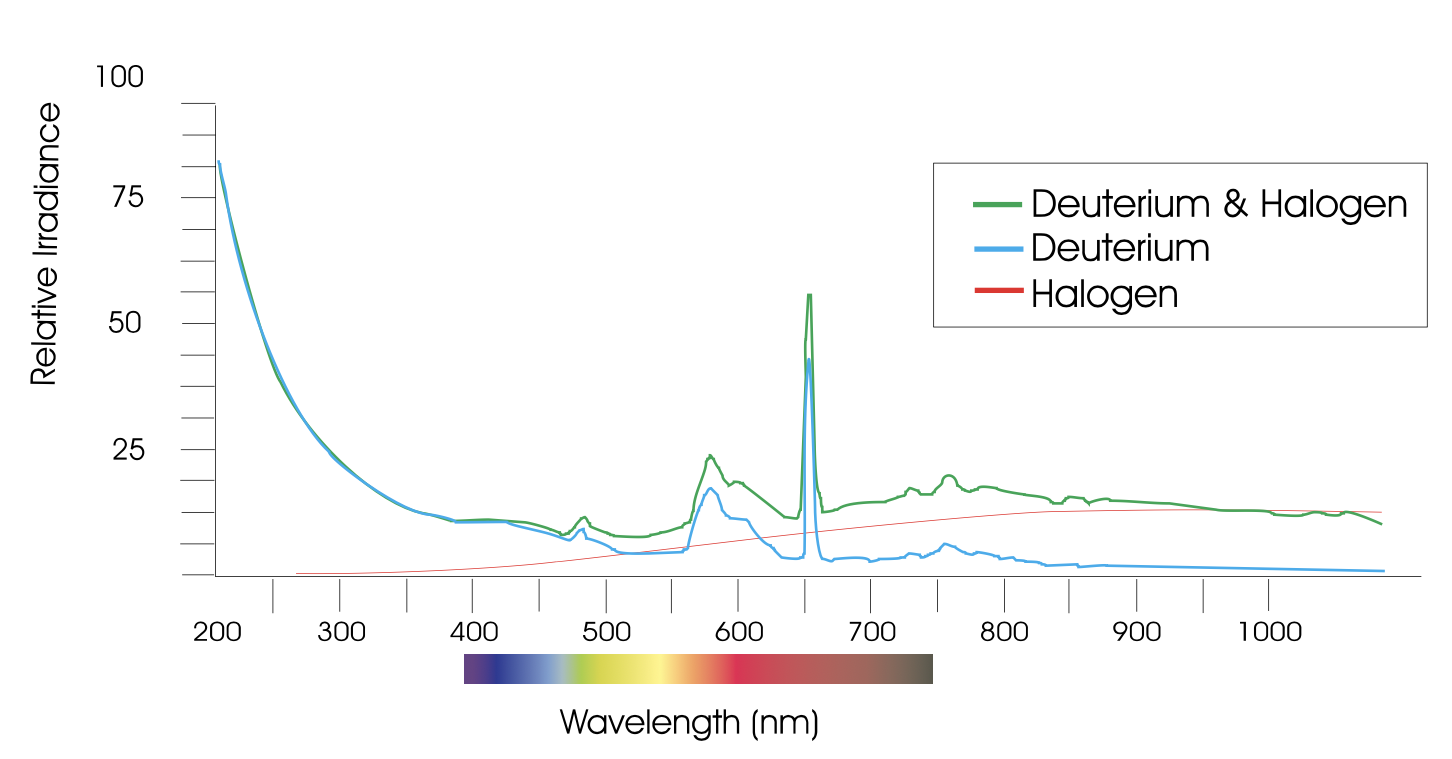
\includegraphics[width=.8\textwidth]{lampenspektrum.png}
    \caption{Spektrum einer Halogenlampe, einer Deuteriumlampe sowie die Kombination der beiden Spektren. Abbildung aus~\cite[]{deuthal}.}
    \label{fig:lampenspektrum}
\end{figure}